\documentclass[conference]{IEEEtran}
\IEEEoverridecommandlockouts

\usepackage[T1]{fontenc}
\usepackage[utf8]{inputenc}
\usepackage{microtype}
\setlength{\emergencystretch}{2em}
\usepackage{amsmath,amssymb,amsfonts,bm}
\usepackage{graphicx}
\usepackage{booktabs}
\usepackage{xcolor}
\usepackage{cite}
\usepackage{enumitem}
\setlist{itemsep=1pt,topsep=3pt}
\usepackage[hidelinks]{hyperref}
\usepackage[capitalize,noabbrev]{cleveref}

\makeatletter
\newcommand{\tabinput}[1]{\@@input #1 }
\makeatother
\newcommand{\p}{\mathbf{p}}
\newcommand{\q}{\mathbf{q}}
\newcommand{\FK}{\mathrm{FK}}
\newcommand{\atantwo}{\operatorname{atan2}}
\newcommand{\code}[1]{\texttt{#1}}

\title{Learning Inverse Kinematics by Imitating a Numerical Solver: Analysis and Improvements on Two 3-DOF Manipulators}

\author{\IEEEauthorblockN{Durgesh S. Reddiyar}
\IEEEauthorblockA{Ira A. Fulton Schools of Engineering\\
Arizona State University, Tempe, AZ, USA\\
dreddiya@asu.edu}}

\begin{document}
\maketitle

\begin{abstract}
To move a robot arm's hand to a target, we need its inverse kinematics (IK): the joint values that place the hand there. A popular shortcut is to train a neural network for IK, using an existing numerical IK solver to create the training examples. We build such a system with the MATLAB Robotics Toolbox and Keras for two simple three-joint arms, and measure how far the arm's hand actually lands from each target. The baseline network misses by a median of about 4\% of the arm's reach, and by more than half the reach for the worst 5\% of targets. Keras's default ``accuracy'' metric still gives it 74\%, because that metric only checks which joint value is largest. Most of the error comes from the training data. The solver often picks different but equally valid solutions for neighbouring targets, so the network has to learn an inconsistent mapping. With consistent, exactly computed labels and a sine--cosine output, the same network becomes $43\times$ more accurate at the median and about $200\times$ more accurate on the hardest targets. Used as a starting guess, it cuts the solver's iterations by $3.5\times$ and always gives the intended solution.
\end{abstract}

\begin{IEEEkeywords}
Inverse kinematics, neural networks, robot manipulators, training data, evaluation metrics.
\end{IEEEkeywords}

\section{Introduction}

A robot arm is controlled through its joints, but tasks are described by where the hand should go. Going from joint values to hand position is easy: it is a fixed chain of rotations and translations called forward kinematics (FK)~\cite{siciliano2009robotics}. Going the other way, from a target position to joint values, is called inverse kinematics (IK) and is harder. A target can have no solution, several, or infinitely many. Some arms have exact formulas for IK~\cite{pieper1968kinematics,diankov2010automated}. Most practical tools instead use iterative solvers that repeatedly adjust the joints until the hand reaches the target~\cite{wampler1986manipulator,nakamura1986inverse,buss2004introduction,sugihara2011solvability,beeson2015trac}.

Neural networks offer another option~\cite{guez1988solution,dsouza2001learning,csiszar2017solving}: once trained, a network gives an answer in one fast, fixed-time step. A common recipe is to pick random targets, label each one by running a numerical solver, and train a network on these examples. The catch is that a target often has several valid solutions, and a network trained on a mix of them can learn their average, which is usually not a solution at all~\cite{jordan1992forward}.

This report builds and analyses such a pipeline for two textbook three-joint arms~\cite{siciliano2009robotics}, using Peter Corke's Robotics Toolbox for MATLAB~\cite{corke1996toolbox,corke2017rvc} and Keras~\cite{chollet2015keras}. We make three contributions:
\begin{itemize}
\item We measure the baseline network by where the hand actually lands, and show that Keras's default accuracy metric hides large errors (\cref{sec:analysis}).
\item We trace the errors to their causes in the training data: inconsistent solution choices, unwrapped angles, and a sampling bug (\cref{sec:analysis}).
\item In a controlled study, we show which fixes matter and by how much, and how a trained network can speed up and steer a numerical solver (\cref{sec:fixes}).
\end{itemize}
The code that produces every number, table, and figure is released with this report.

\section{Related Work}

\emph{Numerical IK.} Most solvers linearise FK at the current guess and take a step towards the target. Plain steps become unstable near singular poses, where the arm loses the ability to move in some direction. Damped least squares and the Levenberg--Marquardt (LM) method add a damping term that keeps steps safe~\cite{wampler1986manipulator,nakamura1986inverse,levenberg1944method,marquardt1963algorithm,sugihara2011solvability}. The toolbox's \code{ikine} function used here is an LM solver~\cite{corke2017rvc}. Two of its properties matter for us. First, which solution it returns depends on the starting guess. Second, it does not wrap angles, so $\theta$ and $\theta+2\pi$ are reported as different answers.

\emph{Learned IK.} Early work trained networks to map positions straight to joint values~\cite{guez1988solution}. Jordan and Rumelhart showed that this averages multiple solutions into invalid ones~\cite{jordan1992forward}. Later methods split the problem into local pieces~\cite{dsouza2001learning,oyama2001modular,csiszar2017solving}, predict structured outputs~\cite{bocsi2011learning}, or learn the full set of solutions with mixture models~\cite{bishop1994mixture}, invertible networks~\cite{ardizzone2019analyzing}, or normalising flows~\cite{ames2022ikflow}. Predicting angles directly is also awkward because of the jump at $\pm\pi$; predicting their sine and cosine avoids it~\cite{zhou2019continuity}.

\section{Robots and Baseline Pipeline}
\label{sec:setup}

\emph{RRR arm.} The first arm has three rotary joints: a base that turns about the vertical axis and two links of length $a_2=a_3=10$ length units (LU). Its hand position is
\begin{equation}
\p=\begin{bmatrix} c_1 r \\ s_1 r \\ a_2 s_2 + a_3 s_{23}\end{bmatrix},\qquad r = a_2 c_2 + a_3 c_{23},
\label{eq:fk}
\end{equation}
where $c_i=\cos\theta_i$, $s_i=\sin\theta_i$, and $c_{23}=\cos(\theta_2+\theta_3)$. The arm can reach any point within 20~LU of its shoulder. Most reachable targets have four solutions: the shoulder can face the target or face away ($\sigma_s=\pm1$), and the elbow can bend up or down ($\sigma_e=\pm1$). With $\rho=\sqrt{p_x^2+p_y^2}$, the exact solutions are
\begin{equation}
\begin{aligned}
\theta_1 &= \atantwo(p_y,p_x) + \tfrac{1-\sigma_s}{2}\pi,\\
c_3 &= \big(\|\p\|^2-a_2^2-a_3^2\big)/(2a_2a_3),\\
\theta_3 &= \atantwo\big(\sigma_e\sqrt{1-c_3^2},\,c_3\big),\\
\theta_2 &= \atantwo(p_z,\,\sigma_s\rho) - \atantwo(a_3 s_3,\,a_2 + a_3 c_3).
\end{aligned}
\label{eq:ik}
\end{equation}
The arm is singular on the vertical axis ($\rho=0$), on the edge of its reach ($\|\p\|=20$), and at the origin, where the elbow folds back on itself.

\emph{RPP arm.} The second arm has a rotary base on a column of height $d_1=5$, a vertical slider $d_2$, and a horizontal slider $d_3$. Its hand is at $\p=[-s_1 d_3,\; c_1 d_3,\; d_1+d_2]^\top$, so its IK has a single solution: $\theta_1=\atantwo(-p_x,p_y)$, $d_2=p_z-d_1$, and $d_3=\rho$.

\emph{Data.} For the RRR arm, 10{,}000 targets are drawn uniformly from the cube $[-15,15]^3$. Each is solved with \code{ikine}, starting from all-zero joints, using a position-only mask and at most 1{,}000 iterations. Targets with no solution are dropped, leaving 9{,}181 examples. For the RPP arm, 10{,}000 targets are drawn with $x\in[0,2\pi]$ and $y,z\in[5,200]$.

\emph{Network.} A fully connected network maps $(x,y,z)$ to three joint values through hidden layers of sizes 32, 64, 128, 256, 256, 256, 128, 128, and 64, with 233{,}027 parameters in total. All layers use ReLU except one sigmoid layer. Training minimises the mean absolute error (MAE) with Adam~\cite{kingma2015adam} (learning rate $10^{-3}$, batch size 768) on an 80:20 train/test split. The RRR network is trained for 20{,}000 epochs.

\emph{How we measure error.} What matters for a task is where the hand ends up. We therefore pass each predicted joint vector through FK and report the \emph{position error} $\|\FK(\hat\q)-\p\|$ in LU. Unlike joint errors, this does not penalise a network for choosing another valid solution or for adding $2\pi$ to an angle.

\emph{Solver re-implementation.} To study the solver at scale, we re-implemented the toolbox's LM method in Python. Each step solves $(J^\top J+\lambda I)\Delta\q=J^\top\mathbf e$, where $J$ is the Jacobian and $\mathbf e$ is the position error. The damping $\lambda$ starts at 0.1, is halved after a successful step, and is doubled after a failed one. The method gives up after 1{,}000 iterations or 100 failed steps in a row.

\section{Analysis of the Baseline}
\label{sec:analysis}

\begin{figure*}[t]
\centering
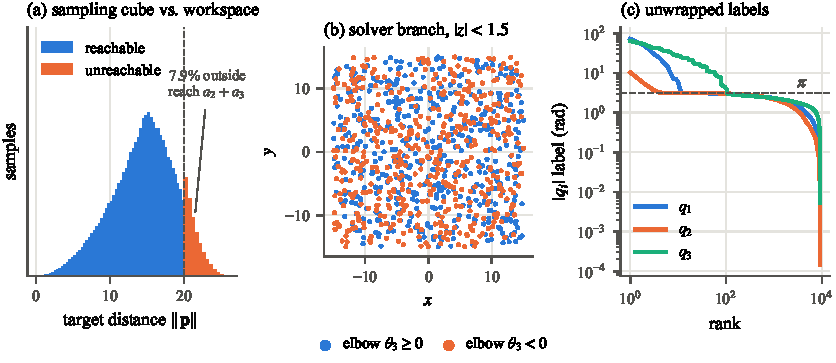
\includegraphics[width=\textwidth]{figures/fig_dataset.pdf}
\caption{Problems in the RRR training data. \textbf{(a)} Distances of targets drawn from the sampling cube. The 7.9\% beyond the arm's 20~LU reach cannot be solved. \textbf{(b)} Elbow direction in the solver's answers for targets near $z=0$. Neighbouring targets often get opposite elbows. \textbf{(c)} Sorted joint labels: some exceed $\pi$ many times over because the solver does not wrap angles.}
\label{fig:dataset}
\end{figure*}

\subsection{Why the solver fails on some targets}
The solver found no answer for 8.2\% of the RRR targets. The reason is simple: the sampling cube's corners lie up to 26~LU away, so 7.9\% of the cube is out of the arm's reach (\cref{fig:dataset}a). Our solver replica failed on 7.8\% of a fresh set of targets, and every failure was out of reach. On reachable targets it never failed and needed at most 51 iterations, so the 1{,}000-iteration limit never mattered. Singular poses did not cause failures either: the kept data come within 0.14~LU of the vertical axis and within $2\times10^{-4}$~LU of the edge of the reach. The solver's answers are accurate, with all position residuals below $5.3\times10^{-3}$~LU.

\subsection{The labels are inconsistent}
Because every solve starts from all-zero joints, which of the four solutions the solver returns depends on where the target lies in a complicated pattern. The nearest training target to a test target is typically only 0.84~LU away, yet it uses the same solution type only 66\% of the time (\cref{fig:dataset}b). In addition, 1.3\% of labels contain an angle outside $(-\pi,\pi]$, up to 71.9~rad (\cref{fig:dataset}c). To the network, these look like completely different answers for nearly identical inputs.

\subsection{The RPP data cover a thin slice of space}
The RPP generator draws the $x$ coordinate from $[0,2\pi]$, an angle range, instead of a position range. As a result, the training targets lie in a thin slab, and the base angle only spans $-49^\circ$ to $0^\circ$, about 14\% of a full turn. Inside this slab the RPP network is accurate, with a median error of 2.1~LU on a workspace of about 200~LU. Outside it, the error grows quickly: for the target $[200,200,100]$ it is 222~LU.

\subsection{Keras's ``accuracy'' is not an IK metric}
For a network with three outputs and an MAE loss, Keras's default \code{'accuracy'} only checks whether the \emph{largest} of the three predicted joint values is in the same position as in the label. It says nothing about the size of the error. The RRR network scores 74.1\% on its test split and 97.3\% on its training split. An RPP network trained on an earlier dataset, with $x\in[0,360]$, scores 91.4\% even though its median position error is 148~LU. Always guessing the most common position of the largest value would already score 81\% there.

\begin{table*}[t]
\centering
\small
\setlength{\tabcolsep}{4pt}
\caption{Trained baseline models. ``Keras acc.'' is Keras's default accuracy metric; ``Maj.'' is the score of always guessing the most common answer. Joint errors are wrapped to $(-\pi,\pi]$. Position errors are in LU; the RRR arm's reach is 20~LU and the RPP workspace is about 200~LU. The last column is the share of targets reached within 1~LU.}
\label{tab:models}
\begin{tabular}{lllrrcrrrr}
\toprule
Model & Arm & Split & Keras acc. & Maj. & Joint error [deg] & \multicolumn{3}{c}{Position error [LU]} & $<1$~LU \\
\cmidrule(lr){7-9}
 & & & [\%] & [\%] & $(q_1,q_2,q_3)$ & median & mean & p95 & [\%] \\
\midrule
\tabinput{tables/tab_models.tex}
\bottomrule
\end{tabular}
\end{table*}

\subsection{How accurate the baseline really is}
\Cref{tab:models} lists all trained models. On test targets, the best RRR network (\code{model20000\_rrr}) lands a median of 0.78~LU from the target, or 3.9\% of the reach. A network that always outputs the average joint values would miss by 23.2~LU, so the baseline clearly learns a lot. The worst cases, however, are bad. The 95th-percentile error is 10.9~LU, more than half the reach, and only 0.5\% of targets are reached within 0.1~LU. The network fits its training targets much better (median 0.50~LU), so it partly memorises them. Most large errors come from picking a different solution type than the label: when the network matches the label's solution type (69\% of targets), its median error is 0.60~LU; when it does not, the median is 1.51~LU and the 95th percentile is 19.7~LU. Errors are also largest near the origin, where the folded elbow makes the joint angles poorly defined. On a typical target such as $\p=[1,4,9]$, the network predicts $[78.8^\circ, 4.4^\circ, 121.2^\circ]$, against the exact solution $[76.0^\circ, 5.1^\circ, 120.7^\circ]$, and misses by 0.23~LU.

\section{Fixing the Training Data}
\label{sec:fixes}

\subsection{Controlled study}
To see which problems matter, we train the same network on the \emph{same} 7{,}344 training targets and change only the labels, the loss, or the output format. The network has three hidden layers of 256 ReLU units. It is trained with Adam for 40k steps (batch size 512, learning rate $2\times10^{-3}$ with cosine decay) in PyTorch~\cite{paszke2019pytorch}, with three random seeds per setting. We test on 20{,}000 new reachable targets. The five label settings are:
\begin{enumerate}[label=(\roman*)]
\item the solver's labels as generated;
\item the same labels with angles wrapped to $(-\pi,\pi]$;
\item exact labels from \cref{eq:ik} with a randomly chosen solution type per target;
\item exact labels that always use the same solution type (shoulder facing the target, elbow up);
\item as (iv), but the network predicts $(\cos\theta_i,\sin\theta_i)$ instead of $\theta_i$.
\end{enumerate}

\begin{table*}[t]
\centering
\small
\setlength{\tabcolsep}{4pt}
\caption{Controlled study on the RRR arm. All runs use the same 7{,}344 training targets and the same network; only the labels, loss, and output format change. Position errors in LU on 20k new reachable targets (mean $\pm$ s.d.\ over 3 seeds). ``$<$0.1'' is the share of targets reached within 0.1~LU, in \%.}
\label{tab:ablation}
\begin{tabular}{lrrrrrr}
\toprule
 & \multicolumn{3}{c}{MAE (L1) loss} & \multicolumn{3}{c}{Squared (L2) loss} \\
\cmidrule(lr){2-4}\cmidrule(lr){5-7}
Labels / output & median & p95 & $<$0.1 & median & p95 & $<$0.1 \\
\midrule
\tabinput{tables/tab_ablation.tex}
\bottomrule
\end{tabular}
\end{table*}

\begin{figure*}[t]
\centering
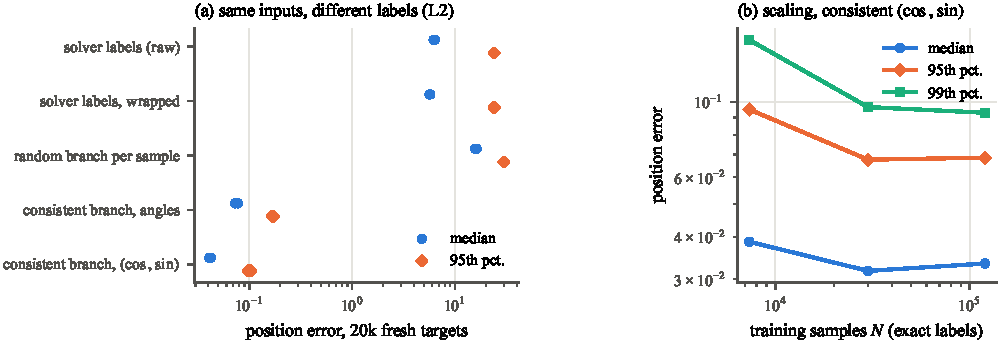
\includegraphics[width=\textwidth]{figures/fig_ablation.pdf}
\caption{\textbf{(a)} Median and 95th-percentile position error for each label setting (L2 loss, three seeds). \textbf{(b)} Error of the improved network as the number of exact training examples grows (mean of three seeds).}
\label{fig:ablation}
\end{figure*}

\Cref{tab:ablation} and \cref{fig:ablation}a show two clear groups. Every setting trained on solver labels or mixed solution types misses by a median of 1.6--16~LU, and its 95th-percentile error is larger than the arm's reach. Every setting trained on one consistent solution type misses by less than 0.075~LU. In more detail:
\begin{itemize}
\item \emph{Mixing solution types is the main problem.} With a random solution type per target, the network misses by 14--16~LU, because it learns averages of valid answers that are not answers themselves.
\item \emph{The loss only matters when labels are mixed.} With solver labels, the MAE loss is $3\times$ better than the squared loss (1.94 vs.\ 6.27~LU), because MAE tends to pick one of the competing answers instead of averaging them. With consistent labels, both losses work well.
\item \emph{Wrapping angles helps a little.} It improves the median by 15\% but leaves the worst cases unchanged.
\item \emph{Sine--cosine outputs finish the job.} They remove the jump at $\pm\pi$ and raise the share of targets reached within 0.1~LU from 72\% to 95\% (L2 loss).
\end{itemize}
With the inputs fixed, consistent labels and a sine--cosine output make the network $43\times$ more accurate at the median (1.94 to 0.045~LU) and $199\times$ more accurate at the 95th percentile (21.9 to 0.11~LU).

\subsection{More data}
Because exact labels are cheap, we can also train on more targets (\cref{fig:ablation}b). With 30{,}000 examples and 60k training steps, the improved network misses by a median of 0.032~LU and reaches 99.1\% of targets within 0.1~LU. Going to 120{,}000 examples gives no further gain, so at this training budget the network, not the data, is the limit. Compared with the baseline on the same new targets, it is $24\times$ more accurate at the median (0.76 to 0.032~LU) and $177\times$ more accurate at the 95th percentile (11.9 to 0.068~LU). It also uses 42\% fewer parameters.

\begin{table}[t]
\centering
\small
\caption{The LM solver on 3{,}000 new reachable targets with different starting guesses. ``Intended'' is the share of answers with the shoulder facing the target and the elbow up. No run failed.}
\label{tab:hybrid}
\begin{tabular}{lrrr}
\toprule
Starting guess & \multicolumn{2}{c}{Iterations} & Intended \\
\cmidrule(lr){2-3}
 & mean & p95 & [\%] \\
\midrule
\tabinput{tables/tab_hybrid_short.tex}
\bottomrule
\end{tabular}
\end{table}

\subsection{The network as a starting guess}
A network can also give the numerical solver its starting point, while the solver still guarantees the final accuracy. \Cref{tab:hybrid} shows the effect. Starting from all-zero joints, the solver needs 15.8 iterations on average, and only 39.5\% of its answers are of the intended type. The baseline network cuts the iterations to 6.2 but does not change which answers come out, since it learned the solver's mixed choices. The improved network cuts the iterations to 4.5 and makes \emph{every} answer the intended type.

\emph{Speed.} In Python on an Apple M1 Pro CPU, the exact formula takes 12.7~\textmu s per target, the improved network 17.8~\textmu s, the baseline network 50.9~\textmu s, and the LM solver 358~\textmu s from zero or 89~\textmu s from the network's guess. For an arm with an exact formula, the formula is fastest and exact. For arms without one, a network is a cheap way to speed up and steer the solver.

\section{Discussion}

\emph{Lessons.} Each problem we found comes from a default that looks harmless on its own. We suggest the following checklist for anyone training an IK network from solver output:
\begin{enumerate}[label=\arabic*.]
\item Sample targets the arm can reach, or sample joints and use FK, which gives exact labels for free.
\item Give every target the same type of solution, or use a model built for multiple answers~\cite{bishop1994mixture,ames2022ikflow}.
\item Wrap angles and predict their sine and cosine.
\item Measure where the hand lands, and report both typical and worst-case errors. Do not use a classification ``accuracy'' for this regression task.
\item Check that input ranges match their units and cover the whole workspace.
\item Keep test data separate, including for example plots, and compare speed against the best available method.
\end{enumerate}

\emph{Limitations.} MATLAB was not available for this analysis, so solver statistics come from our Python re-implementation. It matches the original data in failure rate and solution-type mix, but leaves angles unwrapped more often than the toolbox did. All results on the baseline models use their original weights and data. The study covers two 3-joint arms and position-only IK; larger arms with full position and orientation targets are the natural next step. Timings were measured in Python and are only indicative.

\section{Conclusion}

Training an IK network on a numerical solver's answers seems simple, but the details of the training data decide how well it works. Our baseline network reached targets with a median error of about 4\% of the arm's reach, with much larger worst-case errors, while Keras's default accuracy metric showed none of this. The cause was mainly inconsistent labels: the solver picked different solution types for neighbouring targets and left angles unwrapped. Using one consistent solution type, exact labels, and sine--cosine outputs made the same network $43\times$ more accurate. As a starting guess for a numerical solver, the improved network also cut the iteration count by $3.5\times$ and fixed which solution comes out.

\section*{Acknowledgment}
This work was carried out for MAE~547 (Modeling and Control of Robots) at Arizona State University. The author thanks Rumitkumar Patel and Priyank Patel for their work on the original project. The analysis was carried out with the help of an AI coding assistant. All results were produced by the released scripts, and the author takes full responsibility for the content.

\bibliographystyle{IEEEtran}
\bibliography{refs}

\end{document}
